\documentclass[11pt]{article}

% Language setting
\usepackage[spanish, es-noquoting, es-noshorthands]{babel}
\usepackage[T1]{fontenc}
\usepackage[utf8]{inputenc}
\usepackage{lmodern}
\usepackage{microtype}

% Set page size and margins
\usepackage[letterpaper,top=2cm,bottom=2cm,left=3cm,right=3cm,marginparwidth=1.75cm]{geometry}

% Useful packages
\usepackage{amsmath, amssymb, amsthm, mathtools}
\usepackage{graphicx}
\usepackage[colorlinks=true, allcolors=blue]{hyperref}
\usepackage[capitalise]{cleveref}
\usepackage{enumitem}
\usepackage{multicol}

% Macros for common mathematical symbols
\newcommand{\N}{\mathbb{N}}
\newcommand{\Z}{\mathbb{Z}}
\newcommand{\Q}{\mathbb{Q}}
\newcommand{\R}{\mathbb{R}}
\newcommand{\C}{\mathbb{C}}

\title{\textbf{Guía Álgebra - Práctica 1}}
\author{Lorenzo Durante}
\date{}

\begin{document}
\maketitle

\section{Introducción}
Esta es la resolución de la primera guía de ejercicios de Álgebra 1 para Ciencias de la Computación en la UBA.

\section{Conjuntos}
\subsection{Dado el conjunto \(A = \{ 1, 2, 3\}\), determinar cuáles de las siguientes afirmaciones son verdaderas.}

\begin{enumerate}[label=\roman*)]
    \item \(1 \in A\)
    \item \(\{1\} \subseteq A\)
    \item \(\{2,1\} \subseteq A\)
    \item \(\{1,3\} \in A\)
    \item \(\{2\} \in A\)
\end{enumerate}

\textbf{Resolución}

\begin{enumerate}[label=\roman*)]
    \item \(1 \in A\): el número \(1\) es un elemento que pertenece al conjunto \(A\).
    
    \item \(\{1\} \subseteq A\): el conjunto \(\{1\}\) está contenido en \(A\), ya que todos sus elementos pertenecen a \(A\).
    
    \item \(\{2,1\} \subseteq A\): el conjunto \(\{2,1\}\) es un subconjunto de \(A\), pues tanto \(1\) como \(2\) pertenecen a \(A\).
    
    \item \(\{1,3\} \notin A\): el conjunto \(\{1,3\}\) no es un elemento de \(A\), es decir, \(A\) no contiene a \(\{1,3\}\) como uno de sus elementos.
    
    \item \(\{2\} \notin A\): el elemento \(\{2\}\) no pertenece al conjunto \(A\). 
\end{enumerate}

\subsection{Dado el conjunto \(A = \{1, 2, \{3\}, \{1,2\}\}\), determinar cuáles de las siguientes afirmaciones son verdaderas.}

\begin{multicols}{2}
\begin{enumerate}[label=\roman*)]
    \item \(3 \in A\)
    \item \(\{3\} \subseteq A\)
    \item \(\{3\} \in A\)
    \item \(\{\{3\}\} \subseteq A\)
    \item \(\{1,2\} \in A\)
    \item \(\{1,2\} \subseteq A\)
    \item \(\{\{1,2\}\} \subseteq A\)
    \item \(\{\{1,2\}, 3\} \subseteq A\)
    \item \(\emptyset \in A\)
    \item \(\emptyset \subseteq A\)
    \item \(A \in A\)
    \item \(A \subseteq A\)
\end{enumerate}
\end{multicols}

\textbf{Resolución}
\begin{enumerate}[label=\roman*)]
    \item \(3 \notin A\): es falso ya que el número \(3\) no es un elemento del conjunto \(A\).
    \item \(\{3\} \not\subseteq A\): es falso ya que el elemento \(3\) no está en \(A\).
    \item \(\{3\} \in A\): es verdadero porque el elemento \(\{3\}\) pertenece al conjunto \(A\).
    \item \(\{\{3\}\} \subseteq A\): es verdadero ya que el único elemento de este conjunto es \(\{3\}\) y este pertenece a \(A\). 
    \item \(\{1,2\} \in A\): verdadero, ya que \(\{1,2\}\) pertenece a \(A\).
    \item \(\{1,2\} \subseteq A\): verdadero porque \(1\) y \(2\) pertenecen a \(A\). 
    \item \(\{\{1,2\}\} \subseteq A\): verdadero porque \(\{1,2\}\) pertenece a \(A\). 
    \item \(\{\{1,2\},3\} \not\subseteq A\): falso, ya que \(3\) no pertenece a \(A\). 
    \item \(\emptyset \in A\): falso, ya que \(\emptyset\) no está como elemento dentro de \(A\).
    \item \(\emptyset \subseteq A\): verdadero, ya que el conjunto vacío es subconjunto de todos los conjuntos. 
    \item \(A \in A\): falso, ya que \(A\) no es un elemento de sí mismo.
    \item \(A \subseteq A\): verdadero, ya que todo conjunto es subconjunto de sí mismo.
\end{enumerate}

\subsection{Determinar si \(A \subseteq B\) en cada uno de los siguientes casos.}

\begin{enumerate}[label=\roman*)]
    \item \(A = \{1,2,3\}, \quad B = \{5,4,3,2,1\}\)
    \item \(A = \{1,2,3\}, \quad B = \{1,2,\{3\},-3\}\)
    \item \(A = \{x \in \R \mid 2 < |x| < 3\}, \quad B = \{x \in \R \mid x^2 < 3\}\)
    \item \(A = \{\emptyset\}, \quad B = \emptyset\)
\end{enumerate}

\textbf{Resolución}
\begin{enumerate}[label=\roman*)]
    \item \(A \subseteq B\)
    \item \(A \not\subseteq B\)
    \item \(A \not\subseteq B\)
    \begin{align*}
        A &= [-3,-2] \cup (2,3) \\
        B &= (-\sqrt{3}, \sqrt{3}) \\[6pt]
        &\text{Entonces, } A \nsubseteq B \\
        &\text{Por ejemplo, } -2.5 \in A \;\text{ pero }\; -2.5 \notin B.
    \end{align*}
    \item \(A \not\subseteq B\)
\end{enumerate}

\subsection{Dados los subconjuntos}
\begin{align*}
A &= \{1,-2,7,3\}, \\
B &= \{1,\{3\},10\}, \\
C &= \{-2,\{1,2,3\},3\}
\end{align*}
del conjunto referencial
\[
V = \{1,\{3\},-2,7,10,\{1,2,3\},3\},
\]
hallar
\begin{enumerate}[label=\roman*)]
  \item \(A \cap (B \triangle C)\)
  \item \((A \cap B)\triangle (A \cap C)\)
  \item \(A^{c}\cap B^{c}\cap C^{c}\)
\end{enumerate}

\textbf{Resolución}
\begin{enumerate}[label=\roman*)]
    \item \(A \cap (B \triangle C) = \{1, -2, 3\}\)
    
    Pienso el ejercicio por partes: primero analizo \(B \triangle C\). La diferencia simétrica contiene lo que está en uno u otro, pero no en ambos.
    \begin{align*}
        B &= \{1,\{3\}, 10 \} \\
        C &= \{-2,\{1,2,3\},3\} \\
        B \triangle C &= \{1, \{3\}, 10, -2, \{1,2,3\}, 3\}
    \end{align*}
    Sea \(D = B \triangle C\), evaluemos ahora la intersección entre \(A\) y \(D\).
    \begin{align*}
        A &= \{1,-2,7,3\}, \\
        D &= \{1, \{3\}, 10, -2, \{1,2,3\}, 3\}\\
        A \cap D &= \{1, -2, 3\}
    \end{align*}
    Entonces, el resultado de la intersección es \(\{1, -2, 3\}\).
    
    \item \((A \cap B) \triangle (A \cap C) =  \{1, -2, 3\} \) \\[6pt]
    Primero analizo la primera intersección:
    \begin{align*}
        A &= \{1,-2,7,3\}\\
        B &= \{1, \{3\}, 10\}\\
        A \cap B &= \{1\}
    \end{align*}
    Ahora analizo la segunda intersección:
    \begin{align*}
        A &= \{1, -2, 7, 3\}\\
        C &= \{-2, \{1,2,3\}, 3\}\\
        A \cap C &= \{-2, 3\}
    \end{align*}
    Ahora podemos calcular la diferencia simétrica:
    \begin{align*}
        A \cap B &= \{1\} \\
        A \cap C &= \{-2, 3\} \\
        (A \cap B) \triangle (A \cap C) &= \{1, -2, 3\}
    \end{align*}
    
    \item \(A^{c} \cap B^{c} \cap C^{c} = \emptyset\) \\[6pt]
    El complemento se toma respecto al conjunto referencial \(V\). 
    
    \textbf{Primer complemento:}
    \begin{align*}
        A &= \{1,-2,7,3\}\\
        V &= \{1, \{3\}, -2, 7, 10, \{1,2,3\},3\}\\
        A^{c} &= \{\{3\}, 10, \{1,2,3\}\} 
    \end{align*}
    
    \textbf{Segundo complemento:}
    \begin{align*}
        B &= \{1,\{3\}, 10\}\\
        V &= \{1, \{3\}, -2, 7, 10, \{1,2,3\},3\}\\
        B^{c} &= \{-2, 7, \{1,2,3\}, 3\}
    \end{align*}
    
    \textbf{Tercer complemento:}
    \begin{align*}
        C &= \{-2, \{1,2,3\}, 3\}\\
        V &= \{1, \{3\}, -2, 7, 10, \{1,2,3\}, 3\}\\
        C^{c} &= \{1, \{3\}, 7, 10\}
    \end{align*}

    \textbf{Intersección final:}
    \begin{align*}
        A^{c} &= \{\{3\}, 10, \{1,2,3\}\}\\
        B^{c} &= \{-2, 7, \{1,2,3\}, 3\}\\
        C^{c} &= \{1, \{3\}, 7, 10\}\\
        A^{c} \cap B^{c} \cap C^{c} &= \emptyset
    \end{align*}
\end{enumerate}

\subsection{Dados subconjuntos \(A, B, C\) de un conjunto referencial \(V\), describir 
\((A \cup B \cup C)^{c}\) en términos de intersecciones y complementos, 
y \((A \cap B \cap C)^{c}\) en términos de uniones y complementos.}

\textbf{Resolución}\\[6pt]
Resolvemos con leyes de Morgan: 
\begin{align*}
    (A \cup B \cup C)^{c} &= A^{c} \cap B^{c} \cap C^{c} \\
    (A \cap B \cap C)^{c} &= A^{c} \cup B^{c} \cup C^{c}
\end{align*}

\subsection{Sean \(A\), \(B\) y \(C\) conjuntos. Representar en un diagrama de Venn}

\begin{multicols}{3}
\begin{enumerate}[label=\roman*)]
    \item \((A \cup B^{c}) \cap C\)
    \item \(A \triangle (B \cup C)\)
    \item \(A \cup (B \triangle C)\)
\end{enumerate}
\end{multicols}

Completado en hoja

\subsection{Encontrar fórmulas que describan las partes rayadas de los siguientes diagramas de Venn, utilizando únicamente intersecciones, uniones y complementos.}
\begin{figure}[h!]
    \centering
    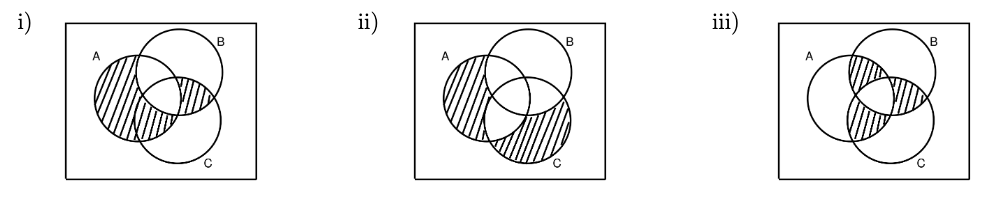
\includegraphics[width=1\textwidth]{image.png}
    \caption{Diagramas de Venn}
    \label{fig:venn}
\end{figure}

\textbf{Resolución}
\begin{enumerate}[label=\roman*)]
    \item \((B^{c} \cap A) \cup (A^{c} \cap C \cap B)\)
    \item \((A \cap B^{c} \cap C^{c}) \cup (C \cap B^{c} \cap C^{c})\) 
    \item \((C^{c} \cap B \cap A) \cup (A^{c} \cap B \cap C) \cup (B^{c} \cap A \cap C)\)
\end{enumerate}

\subsection{Hallar el conjunto \(P(A)\) de partes de \(A\) en los casos}
\begin{multicols}{3}
    \begin{enumerate}[label=\roman*)]
        \item \(A = \{1\}\)
        \item \( A = \{a, b\}\)
        \item \(A = \{1, \{1, 2\}, 3\}\)
    \end{enumerate}
\end{multicols}

\textbf{Resolución}

\begin{enumerate}[label=\roman*)]
    \item \(P(A) = \{\emptyset, \{1\}\}\)
    \item \(P(A) = \{\emptyset, \{a\}, \{b\}, \{a, b\}\}\)
    \item \(P(A) = \{\emptyset, \{1\}, \{\{1,2\}\}, \{3\}, \{1, \{1,2\}\}, \{1, 3\}, \{\{1,2\}, 3\}, \{1, \{1,2\}, 3\}\}\)
\end{enumerate}

\subsection{Sean \(A\) y \(B\) conjuntos. Probar que \(P(A) \subseteq P(B) \Leftrightarrow A \subseteq B\)}

\subsection{Sean \(p, q\) proposiciones. Verificar que las siguientes expresiones tienen la misma tabla de verdad para concluir que son equivalentes.}

\begin{enumerate}[label=\roman*)]
\item \(p \Rightarrow q\), \quad \(\sim q \Rightarrow \sim p\), \quad \(\sim p \lor q\) \quad y \quad \(\sim (p \land \sim q)\).

Esto nos dice que podemos demostrar una afirmación de la forma \(p \Rightarrow q\) probando en su lugar 
\(\sim q \Rightarrow \sim p\) (es decir \textit{demostrando el contrarrecíproco}), 
o probando \(\sim (p \land \sim q)\) (esto es una \textit{demostración por reducción al absurdo}).

\item \(\sim (p \Rightarrow q)\) \quad y \quad \(p \land \sim q\).

\end{enumerate}

\textbf{Resolución}
\begin{enumerate}[label=\roman*)]
   \item \[
\begin{array}{|c|c|c|}
\hline
p & q & p \rightarrow q \\
\hline
V & V & V \\
V & F & F \\
F & V & V \\
F & F & V \\
\hline
\end{array}
\]

\[
\begin{array}{|c|c|c|}
\hline
p & q & \neg q \rightarrow \neg p \\
\hline
V & V & V \\
V & F & V \\
F & V & F \\
F & F & V \\
\hline
\end{array}
\]

\[
\begin{array}{|c|c|c|}
\hline
p & q & \neg p \and q \\
\hline
V & V & V \\
V & F & F \\
F & V & V \\
F & F & V \\
\hline
\end{array}
\]

\[
\begin{array}{|c|c|c|}
\hline
p & q & \neg (p \land \neg q) \\
\hline
V & V & V \\
V & F & F \\
F & V & V \\
F & F & V \\
\hline
\end{array}
\]

Todas las tablas tienen la misma tabla de verdad por ende, son equivalentes. 

\item 
\[
\begin{array}{|c|c|c|}
    \hline
    p & q & \neg(p \rightarrow q) \\
    \hline
    V & V & F \\
    V & F & V \\
    F & V & F \\
    F & F & F \\
    \hline
\end{array}
\]

\[
\begin{array}{|c|c|c|}
    \hline
    p & q & p \land \neg q \\
    \hline
    V & V & F \\
    V & F & V \\
    F & V & F \\
    F & F & F \\
    \hline
\end{array}
\]
Es equivalente. 
\end{enumerate}

\subsection{Hallar contraejemplos para mostrar que las siguientes proposiciones son falsas.}

\begin{enumerate}[label=\roman*)]
    \item $\forall a \in \mathbb{N}, \; \frac{a-1}{a}$ no es un número entero.
    \item $\forall x, y \in \mathbb{R}$ con $x, y$ positivos, $\sqrt{x+y} = \sqrt{x} + \sqrt{y}$.
    \item $\forall x \in \mathbb{R}, \; x^2 > 4 \Rightarrow x > 2$.
\end{enumerate}

\textbf{Resolución}
\begin{enumerate}[label=\roman*]
    \item 
\end{enumerate}
\end{document}